\documentclass[11pt]{article}
\usepackage[utf8]{inputenc}
\usepackage[T1]{fontenc}
\usepackage{grffile}
\usepackage{longtable}
\usepackage{wrapfig}
\usepackage{rotating}
\usepackage[normalem]{ulem}
\usepackage{amsmath}
\usepackage{textcomp}
\usepackage{amssymb}
\usepackage{capt-of}
\usepackage{hyperref}
\hypersetup{colorlinks=true, linkcolor=magenta, citecolor=cyan}
\setlength{\parindent}{0in}
\usepackage[margin=1in]{geometry}
\usepackage[english]{babel}
\usepackage{mathtools}
\usepackage{palatino}
\usepackage{fancyhdr}
\usepackage{sectsty}
\usepackage{engord}
\usepackage{parskip}
\usepackage{minted}
\usepackage{graphicx}
\usepackage{subcaption}
\usepackage{setspace}
%\usepackage[center]{caption}
\usepackage{placeins}
\usepackage{color}
\usepackage{amsmath}
\usepackage{bm}
\usepackage{todonotes}
\usepackage{pdfpages}
% \titlespacing*{\subsection}{0pt}{5.5ex}{3.3ex}
%\titlespacing*{\section}{0pt}{5.5ex}{1ex}
\usepackage{natbib}
\setcitestyle{authoryear,aysep={,}}

\author{Luis Antonio Ortega Andrés\\Antonio Coín Castro}
\date{\today}
\title{DeepFakes Detection Lab - Report}
\hypersetup{
 pdfauthor={Luis Antonio Ortega Andrés, Antonio Coín Castro},
 pdftitle={},
 pdfkeywords={},
 pdfsubject={},
 pdflang={English}
 }

\begin{document}

\maketitle

\section*{Task 1: intra-database analysis}

\textit{The goal of this task is to develop and evaluate DeepFake detection systems over the same database. In this task, you should use only the UADFV database, which is divided into \texttt{development} and \texttt{evaluation} datasets.}

The notebook associated with this task is \texttt{Task1-2.ipynb}.

\textbf{a)} \textit{Provide all details (including links or references if needed) of your proposed DeepFake detection system.}

Our DeepFake detection system consists on the following modules:
\subsection*{Preprocessing}

First of all, the given images from UADFV have been preprocessed following these steps:
\begin{enumerate}
  \item The data is loaded using \texttt{Keras}' \texttt{flow\_from\_directory} function \citep{chollet2015keras}, so that we don't have to keep all images in memory while training our model. We resize each image to a resolution of $768\times 768$.
  \item We use the MTCNN face detector \citep{zhang2016joint} in order to crop the section of the image that contains the face. The aim of this phase is to erase those parts of the image that are not relevant for our classification task.
  \item We add random noise to the images as a form of regularization, to force our classifier to learn more relevant features. More precisely, we randomly decide wether the image is slightly blurred using a Gaussian filter from OpenCV \citep{opencv_library}, or simply perturbed by Gaussian noise. Each of these outcomes is equally likely and every image goes through one or the other, but never both. Note that these perturbations are only applied to training samples and not to the evaluation images.
\end{enumerate}

\subsection*{Feature extraction}

We decided that the best way of extracting features from the faces was \texttt{dlib}'s 68-point face landmark detector \citep{dlib09}. For each (cropped) face image, we obtain the spatial position of the 68 landmarks, and our final feature vector is composed of the gray-scale intensities of these landmarks. We then center each feature vector to have zero mean.

We also considered the possibility of applying PCA for dimensionality reduction, but since we wanted to try both approaches, we delegated this decision to the actual training step.

\subsection*{Classifier}

The final step of our model is a machine learning model that acts as a classifier to which the feature vectors are fed for training. At first we considered four distinct families of models for this job: \textbf{Linear SVM}, \textbf{SVM with RBF kernel}, \textbf{2-layer perceptron} and \textbf{Logistic Regression} models. The process by which a final classifier was selected can be seen on the next section.

\textbf{b)} \textit{Provide all details of the development/training procedure followed and the results achieved using the development dataset of the UADFV database. Show the results achieved in terms of Receiver Operating Characteristic (ROC) curve and Area Under the Curve (AUC).}

For the training procedure we performed a hyperparameter grid search using \texttt{Sklearn}'s API \citep{sklearn_api}, in which each family of classifiers mentioned above is tested with a wide range of possible hyperparameters to maximize the AUC metric. For example, the number of hidden layers considered for the MLP are \( \{(50), (100), (50, 50), (100, 100)\} \), and the linear SVM regularization term \( C \) varies from \( 10^{-3} \) to \( 10^{3} \) with 40 equidistant steps. To make the process fair, we employ \textbf{5-fold cross validation} to select the best hyperparameters for each model, and in the end we select the model that achieved the highest cross-validated AUC. Note that each family of classifiers is trained using the same folds, so the results are comparable.

Before completing the training pipeline, we added the possibility to train each classifier \textbf{with and without PCA reduction}, to see whether it would have a positive impact on the final result. The fraction of explained variance to be retained was also an hyperparameter, whose search space was $\{0.90, 0.95, 0.99\}$. An important detail is that the data is first standardized to have zero mean and unit variance, since we observed that the performance of the classifiers was noticeably better after this normalization.

The best models of each family after running the grid search are shown in Table \ref{tab:t1}, along with their cross-validated AUC scores.

\begin{table}[H]
  \centering
  \begin{tabular}{llll}
    \textbf{Model}      & \textbf{PCA} & \textbf{Parameters} & \textbf{AUC (CV)} \\ \hline
    SVM RBF             & No &      \( C = 1.6681, \, \gamma = 0.0167\)  &     \( {\color{blue!80!black}{0.9937}} \)       \\
    SVM Linear          & No &   \(  C = 0.0174 \)   &   \( 0.9186 \)   \\
    MLP                 & No  &  \(\alpha=0.2154, \,size=(100, 100) \)     &    \(  0.9883 \)          \\
    LR & No & \( C = 0.1624 \) &    \( 0.9180 \)
    \end{tabular}
    \caption{Results of the hyperparameter tuning phase.}
    \label{tab:t1}
  \end{table}

As we can see, the best performing model was the \textbf{non-linear SVM with RBF kernel using the raw features}, and this is the model that we choose as our final classifier (with the optimized parameters found). An interesting thing to note is that PCA was discarded on every model, probably because the number of raw features considered is not very high. The results of evaluating our chosen model on the whole development set can be seen on Figure \ref{fig:t1-roc-train}.

\begin{figure}[h!]
  \centering
  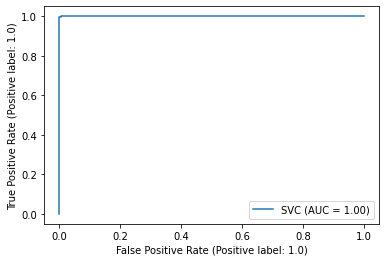
\includegraphics[width=.6\textwidth]{img/1-roc-UADFV-train}
  \caption{ROC curve and AUC value on UADFV's development set.}
  \label{fig:t1-roc-train}
\end{figure}

\textbf{c)} \textit{Describe the final evaluation of your proposed DeepFake detection system and the results achieved using the evaluation dataset (not used for training). Show the results achieved in terms of ROC curve and AUC. Provide an explanation of your results.}

Having chosen our model, we simply evaluate it on the previously unseen evaluation set of UADFV database, and the results can be seen in Figure \ref{fig:t1-roc-test}. We obtain an AUC of $0.95$, quite close to the perfect score of $1.0$. We can say that we have succeeded in this task, since our model has learned to detect DeepFakes on the UADFV database at different threshold while avoiding overfitting.

\begin{figure}[h!]
  \centering
  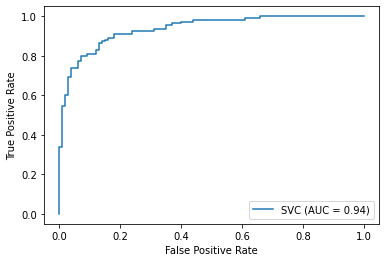
\includegraphics[width=.6\textwidth]{img/1-roc-UADFV}
  \caption{ROC curve and AUC value on UADFV's evaluation set.}
  \label{fig:t1-roc-test}
\end{figure}

\subsection*{Other approaches and failed attempts}

\begin{enumerate}
  \item We considered extracting features using an image destriptor such as SURF or SIFT, and then following the Bag of Visual Words technique. However, the results obtained were worse, so we discarded this approach.
  \item Along with the landmarks intensity, we made some attempts at using the the landmarks locations as features, but this resulted in overfitting. As a regularization technique, we centered those locations (substracting the mean) in order to make them location invariant. The performance improved a bit but in the end we decided to stick to the face landmarks only.
  \item At one point, MTCNN did not correctly detect the faces for every image, and during training we decided to simply skip these images. However, since we cannot skip test cases, we decided that an image with no face detected would be assumed to have the same features as the last image with the same label. In the end we solved the underlying problem (by resizing the input images), but we left all the code checks just in case they were needed in the future.
  \item More models were tested in the grid search, such as Random Forests and other boosting techniques. However, they performed so poorly compared to the rest that we decided not to include them in the final report.
\end{enumerate}

\section*{Task 2: inter-database analysis}

\textit{The goal of this task is to evaluate the DeepFake detection system developed in Task 1 with a new database (not seen during the development/training of the detector). In this task, you should use only the Celeb-DF. You only need to evaluate your fake detector developed in Task 1 over the \texttt{evaluation} dataset of Celeb-DF, not train again with them.}

The notebook associated with this task is \texttt{Task1-2.ipynb}.

\textbf{a)} \textit{Describe the results achieved by your DeepFake detection system developed in Task 1 using the evaluation dataset of the Celeb-DF database. Show the results achieved in terms of ROC curve and AUC. Provide an explanation of your results in comparison with the results of Task 1.}

We evaluate the model established in the previous task (SVM with RBF kernel and optimized hyperparameters) on the evaluation set of Celeb-DF. The results achieved can be seen in Figure \ref{fig:t2}.

\begin{figure}[h!]
  \centering
  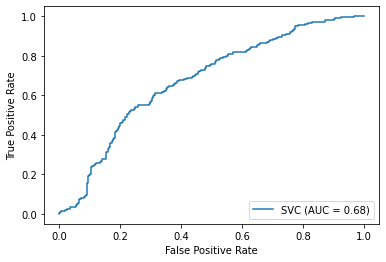
\includegraphics[width=.6\textwidth]{img/2-roc-celeb}
  \caption{ROC curve and AUC value on Celeb-DF's evaluation set.}
  \label{fig:t2}
\end{figure}

We obtain an AUC of 0.64, which is considerably lower than the one achieved in the previous task. This behaviour makes sense, considering that the training dataset was less challenging than this one, in the sense that the deepfakes were more easily spotted by a human. In the UADFV dataset there were usually vertical and horizontal strips surrounding the place where the face exchange had taken place, and in this new dataset deepfakes have a higher quality and do not show such markings. In short, our detection model scales poorly to this dataset because the data in which it was trained \textbf{is not representative enough} of this new evaluation set.


\section*{Task 3: inter-database proposal}

\textit{The goal of this task is to improve the DeepFake detection system originally developed in Task 1 in order to achieve better inter-database results. You must consider the same evaluation dataset as in Task 2 (i.e. the \texttt{evaluation} dataset of the Celeb-DF database).}

\textbf{a)} \textit{Describe the improvements carried out in your proposed DeepFake detection system in comparison with Task 1.}

For this task, we followed different approaches in order to find and optimise the most suitable technique for this problem. For every of the following aproaches the \textbf{training dataset} was composed of \( 1823 \) \( 160\times 160 \) face samples obtained via \texttt{mtcnn}. To build this training set we used the full given set of UADFV and several samples (around \( 1000 \)) of \textbf{DeepfakeTimit} and \textbf{vidTimit} (\cite{sanderson2009multi}). As DeepfakeTimit is composed of videos, we a \texttt{python script} (\texttt{TIMIT\_data\_preprocess.py}) in order to take frames from such videos. As these dataset have pretty low diversity (only 32 different persons appear on the videos), we decided to not to take all the samples we could, but get a random sample of both real and fakes images while we cropped the \( 160 \times 160 \) face image (\texttt{Face\_detector\_splitter.py}).

On the other hand, the \textbf{evaluation dataset} is composed of the \( 160 \times 160 \) faces of each sample in the given \texttt{Celeb-DF} dataset. 

Both, training and evaluation sets can be found in (files).

\subsection*{Train the same model with more data}

In this attempt, we aimed to check how the best model of the previous task behaved in this one. This approach is used to set a \emph{starting line} to be compared to the subsequent attempts.

The procedure was simple and can be seen in \texttt{Task3\_ML.ipynb}, we reused part of the code developed for the previous task and create a pipeline with the optimal classifier. The AUC obtained using this approach is 0.67.

\subsection*{Consider alternative features}

In this approach we intended to use \texttt{Facenet} (\cite{Schroff_2015}) to obtain a more representative set of features compared to the ones computed by \texttt{dlib}. To this end, we took a pre-trained model of Facenet that performed an embedding to \( 128 \) features and used these to train and cross-validate the same models considered in Task 1.

As a result, the chosen model was a RBF SVM with regularization term \( C = 4.6415 \) and kernel length \( \gamma = 0.01668 \), giving an AUC of \( 0.7 \) on the evaluation dataset.

This approach can be consulted in \texttt{Task3\_Facenet.ipynb}.

\subsection*{Train a deep learning model from scratch}


In this attempt we wanted to take advantage of the increased number fo samples in the training dataset to use a \emph{not so deep} convolutional network for the classification task. We considered two blocks of convolution-activation-dropout and 2 fully connected layers for the model.  

In the end, after tunning the parameters for a while, the model either overfitted to the training dataset or did not learn at all. The general structure can be found at \texttt{Task3\_DL.ipynb}

\subsection*{Fine-tune a pre-trained deep learning model}


As out last attempt, we aimed to fine-tune a pre-trained deep neural network. To this end, we tested several well-known models as VGG19, XceptionNet..., dropped the last layers and used a pair of fully connected layers to make the classification. The aim is to use the higher feature extraction  potential of those pre-trained models and make a classification with them.

In order to fine-tune de model, we froze the layers from the pre-trained model and trained the full one just a few epochs. The objective is that the final new layers learn to use the features to the new classification task. After this, we defroze all the layers and trained the full model for several epochs.

In the end, the pre-trained model that performed the best is VGG19 (\cite{simonyan2015deep}) with 3 initial epochs followed by another 15 (\texttt{Task3\_Finetune.ipynb}).

\textbf{b)} \textit{Describe the results achieved by your enhanced DeepFake detection system over the final evaluation dataset. Show the results achieved in terms of ROC curve and AUC. Provide an explanation of your results in comparison with the results of Task 2.}

Final graph (AUC 0.81).

\begin{figure}[h!]
  \centering
  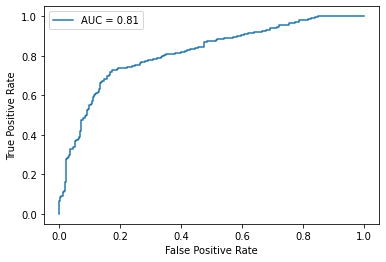
\includegraphics[width=.6\textwidth]{img/3-finetune-roc-celeb}
  \caption{ROC curve and AUC value on Celeb-DF's evaluation set for our enhanced model.}
  \label{fig:t3}
\end{figure}

\textbf{c)} \textit{Indicate the conclusions and possible future improvements}.

Not enough data; finetuning is essential; Deep learning outperforms classical approaches when used appropriately.

face align, face masks, one-to-many, many-to-one, (eye, mouth, teeth,... more fine grained approach to feature extraction.)

%%%%%%%%%%%%%%%%
%% Bibliography
%%%%%%%%%%%%%%%%

\bibliographystyle{authordate1}
\bibliography{bibliography}

\end{document}
